Electric energy is often described as flowing through wires, like water through a pipe. This analogy is common but misleading. It treats energy as a substance carried by electrons moving from source to device. But in reality, electrons inside a conductor move slowly. Their average drift velocity under a typical voltage is only a few millimeters per second. What moves quickly is not the charge, but the influence — the disturbance in the electromagnetic field that propagates through space. A better analogy, if still inaccurate, is a wave traveling across the surface of a pond: the water does not move forward, but the wave does. In the same way, electric energy is transmitted by the wave-like interaction of fields, not by the displacement of material particles.

This effect is visible also in static electricity. When two materials are rubbed together, electrons are transferred from one to the other, creating a separation of charge. No current flows, yet a strong electric field appears in the surrounding space. That field can exert forces, store energy, and discharge when a conductive path is introduced. The important quantity is not how fast electrons move, but how their arrangement defines the electric field, and how that field interacts with its magnetic counterpart.

When a switch is closed in a circuit, electrical devices respond almost instantly. This is not because electrons move from one end of the wire to the other, but because the electromagnetic fields associated with the circuit are established nearly simultaneously throughout its geometry. A voltage sets up an electric field $\mathbf{E}$ along the wire, and a current produces a magnetic field $\mathbf{B}$ encircling it. These fields extend beyond the physical surface of the conductor, occupying the surrounding space and determining the actual path along which energy travels.

The mathematical structure of this behavior is formalized in Maxwell’s equations. Before Maxwell, electric and magnetic phenomena were treated separately: electric fields originated from static charges, and magnetic fields from moving charges — that is, from currents. These laws worked well for static situations but failed in time-varying regimes. Maxwell identified a critical gap in Ampère’s law. According to its original form, a magnetic field was produced only by conduction current. But this led to contradictions in cases where the electric field changed in time but no actual current flowed — such as inside a capacitor during charging. Maxwell resolved the inconsistency by introducing the concept of displacement current: the idea that a changing electric field $\partial \mathbf{E}/\partial t$ acts like a current, generating a magnetic field even in the absence of moving charge.

This single correction completed the system. By adding the displacement current term, Maxwell’s equations predicted that electric and magnetic fields can sustain each other in time: a changing electric field $\mathbf{E}$ generates a magnetic field $\mathbf{B}$, and a changing $\mathbf{B}$ regenerates $\mathbf{E}$. This mutual coupling leads to wave propagation even in the absence of charge or current. The speed of this wave is determined by vacuum properties: permittivity $\varepsilon_0$ and permeability $\mu_0$, with $c = 1/\sqrt{\varepsilon_0 \mu_0}$. This speed matched the measured speed of light in vacuum, confirming that classical electromagnetic waves propagate at the same rate. This identification led to the interpretation of light, within classical physics, as an electromagnetic wave solution to Maxwell’s equations.

The physical picture is this: an oscillating $\mathbf{E}$ field produces a perpendicular, time-varying $\mathbf{B}$ field, which in turn regenerates $\mathbf{E}$. The fields constitute the energy themselves. To compute energy flow, the magnetic field $\mathbf{B}$ must be normalized by the vacuum permeability: $\mathbf{H} = \mathbf{B} / \mu_0$. This ensures that both $\mathbf{E}$ and $\mathbf{H}$ are expressed in compatible units when evaluating energy flux. The resulting Poynting vector, $\mathbf{S} = \mathbf{E} \times \mathbf{H}$, describes the instantaneous direction and intensity of electromagnetic energy transport. It has units of power per unit area (W/m$^2$) and is always perpendicular to both fields.

In some branches of theoretical physics, including high-energy and relativistic field theory, natural units are adopted in which $\varepsilon_0 = \mu_0 = 1$, or equivalently $c = 1$. In these units, $\mathbf{B}$ and $\mathbf{H}$ become indistinct.

\begin{tcolorbox}[title={Electromagnetic Quantities: Definitions, Units, and Dimensions}, 
colback=gray!6, colframe=black!50, fonttitle=\bfseries, coltitle=black, boxrule=0.4pt, arc=1pt, 
left=6pt, right=6pt, top=4pt, bottom=4pt]

\renewcommand{\arraystretch}{1.3}
\begin{tabularx}{\textwidth}{>{\bfseries}l >{\bfseries}l X c c}
\textbf{Symbol} & \textbf{Name} & \textbf{Meaning} & \textbf{SI Units} & \textbf{Dimensions} \\ \hline

% Group: Field Quantities
$\mathbf{E}$ & Electric field & Force / unit test charge & V/m & $\mathrm{MLT^{-3}I^{-1}}$ \\
$\mathbf{B}$ & Magnetic field & Force / unit charge / velocity & T = V·s/m$^2$ & $\mathrm{MT^{-2}I^{-1}}$ \\
$\mathbf{H}$ & Magnetic intensity & Rescaled mag. field: $\mathbf{B} = \mu \mathbf{H}$ & A/m & $\mathrm{IL^{-1}}$ \\

% Group: Constants
$\varepsilon_0$ & Vacuum permit. & Field / unit charge density & F/m & $\mathrm{M^{-1}L^{-3}T^4I^2}$ \\
$\mu_0$ & Vacuum permea. & Field / unit current density & H/m & $\mathrm{MLT^{-2}I^{-2}}$ \\

% Group: Derived Propagation Quantities
$\mathbf{S}$ & Poynting vector & Energy flow / unit area & W/m$^2$ & $\mathrm{MT^{-3}}$ \\
$u$ & Energy density & Energy / unit volume & J/m$^3$ & $\mathrm{ML^{-1}T^{-2}}$ \\
$Z_0$ & Vacuum impedance & Ratio of electric to magnetic & $\approx 377\ \Omega$ & $\mathrm{ML^2T^{-3}I^{-2}}$ \\
$c$ & Speed of light & Wave speed in vacuum & m/s & $\mathrm{LT^{-1}}$ \\

% Group: Base Electrical Units
$A$ & Ampere & Charge flow / unit time & C/s & $\mathrm{I}$ \\
$F$ & Farad & Charge / unit voltage & C/V & $\mathrm{M^{-1}L^{-2}T^4I^2}$ \\
$W$ & Watt & Energy / unit time & J/s & $\mathrm{ML^2T^{-3}}$ \\

% Optional: Basic Circuit Quantities
$Q$ & Charge & Net electric quantity & C & $\mathrm{IT}$ \\
$V$ & Voltage & Energy / unit charge & V = J/C & $\mathrm{ML^2T^{-3}I^{-1}}$ \\
$R$ & Resistance & Voltage / unit current & $\Omega = V/A$ & $\mathrm{ML^2T^{-3}I^{-2}}$ \\

\end{tabularx}
\end{tcolorbox}






In a simple conducting wire, the electric field $\mathbf{E}$ points radially outward, the magnetic field $\mathbf{B}$ encircles the wire azimuthally, and the Poynting vector $\mathbf{S}$ points along the wire. But this power flow occurs in the surrounding space, not within the conductor itself. The role of the wire is to establish boundary conditions that constrain and guide the fields. The actual transfer of energy happens in the fields that occupy the space around the wire rather than the motion of charge through its interior.

Now for the electrons. Before electrons were understood as discrete particles, early models of electricity imagined it as a continuous substance flowing through wires, like water through a pipe. In this mechanical analogy, the conductor acted as a passive conduit, and the observable effects of voltage and current were attributed to the movement of an invisible, uniform electrical fluid. This picture offered no means of predicting resistance, current strength, or temperature dependence, and it could not account for microscopic structure.

Before electrons were understood as discrete particles, electricity was commonly described using fluid analogies. The wire served as a pipe, and the electric current was imagined as a continuous substance moving through it. This model offered some intuition for the flow of charge but could not account for resistance, material dependence, or thermal effects. It lacked a microscopic description of matter and provided no means to calculate the behavior of specific materials under applied voltage.

In 1900, Paul Drude introduced a kinetic theory of conduction that treated electrons as classical particles moving freely between instantaneous collisions with heavy, stationary ions in a metallic lattice. Under an applied electric field, the electrons acquired a small net drift velocity superimposed on their thermal motion, giving rise to a steady current. This model successfully reproduced Ohm’s law and introduced the concept of mean free path. However, it relied on Maxwell–Boltzmann statistics and treated electrons as distinguishable particles in thermal equilibrium. These assumptions, though reasonable for a dilute gas, led to contradictions when applied to dense electron systems in metals.

One of the first major contradictions came from measurements of the electronic contribution to specific heat. Classical theory, using the equipartition theorem, predicted that each electron would contribute $\tfrac{3}{2}k_B$ to the heat capacity. In metals with high electron density, this led to values far above what was observed. Calorimetry showed that the actual electronic contribution was over a hundred times smaller than predicted, especially at low temperatures. The discrepancy could not be resolved by adjusting parameters within the classical framework. It indicated that the majority of electrons were somehow prevented from gaining thermal energy, contrary to the assumptions of the Drude model.

A second failure arose from the relation between electrical and thermal conductivity. According to the Wiedemann–Franz law, the ratio $L = \kappa / (\sigma T)$ should be constant across temperatures and materials, provided that the same electrons carry both charge and heat. Experiments showed that this Lorenz number varied significantly with temperature, particularly in the low-$T$ regime. This variation implied that energy and charge transport were not governed by identical carriers or scattering mechanisms. Electrostatic experiments revealed another inconsistency. When an electric field was applied outside a conductive enclosure, no field was detected inside. The Drude model offered no mechanism for this rapid field suppression, since it treated electrons as isolated particles without collective behavior.

Further contradictions came from temperature-dependent resistivity. Drude’s model predicted that resistivity should increase linearly with temperature due to more frequent electron–ion collisions. In practice, resistivity curves showed clear deviations from linearity, especially at low temperatures where resistance often plateaued or decreased. High-purity metals with large crystalline domains exhibited behavior that depended sensitively on defect density, lattice structure, and impurity concentration. These features played no role in Drude’s theory, which treated the lattice as a uniform background. The observed dependence on structural details suggested that new scattering mechanisms and quantum restrictions were at play.

In 1912, Peter Debye addressed the failures of the Drude model by incorporating lattice dynamics into the theory of conduction. Rather than treating ions as fixed scattering centers, he modeled them as thermally vibrating masses whose motion becomes increasingly pronounced with temperature. These vibrations were treated as quantized normal modes — modernly termed phonons — which represent collective oscillations of the atomic lattice. Unlike localized particle collisions, phonons describe delocalized, wave-like excitations that span the crystal and interact coherently with conduction electrons. As the temperature rises, the number and amplitude of accessible phonon modes increase, leading to more frequent electron–phonon collisions and higher resistivity. This framework introduced a temperature-dependent scattering mechanism that aligned more closely with observed trends in metallic resistance.

The phonon-based model explained key features of resistivity across a wide temperature range. At high temperatures, the increased phonon population leads to a nearly linear growth in resistivity, consistent with the empirical behavior of most metals. At low temperatures, however, the phonon modes freeze out, drastically reducing scattering rates. This accounts for the saturation or decline of resistivity observed in cryogenic conditions. The model also clarified why high-purity metals, with fewer structural defects, exhibited more pronounced temperature effects: in such systems, electron–phonon scattering dominates, and the absence of impurity scattering allows the temperature dependence to emerge more clearly. Debye’s formulation provided a unified account of resistive behavior that classical collision models could not reproduce.

Debye also introduced the idea of electrostatic screening in metals. When an external electric field is applied to a conductor, the conduction electrons respond as a collective, redistributing themselves to cancel the field within a short distance from the surface. This rearrangement suppresses internal electric fields and confines any applied potential to a thin boundary layer. The characteristic length over which this suppression occurs is now called the Debye length. It depends on the electron density and temperature, and is typically on the order of nanometers in metals. This concept provided a theoretical basis for the empirical fact that conductors exhibit perfect shielding under static conditions. It also reframed the conductor as an electronically responsive medium governed by collective charge motion rather than isolated particle dynamics.

While Debye focused on the quantized behavior of the lattice, in 1928, Arnold Sommerfeld turned to the electron gas itself. Debye’s model resolved key thermal anomalies by treating lattice vibrations as phonons and introducing collective screening, but it still relied on classical statistics for the electrons. Sommerfeld’s contribution was to replace the classical electron gas with a quantum one, governed by the Pauli exclusion principle. In this revised model, electrons occupy discrete quantum states and fill all available levels up to the Fermi energy. Only those near this surface can change state when a weak external field is applied. This restriction explains why most electrons do not contribute to conduction or specific heat, despite their large individual velocities. It also accounts for the small but nonzero electronic heat capacity and the weak temperature dependence of conductivity in pure metals. Sommerfeld’s approach completed the redefinition of conduction: not as thermal drift through a static lattice, but as the quantum response of a filled electron sea to external perturbation.

The Sommerfeld model resolved the longstanding discrepancy in the electronic specific heat. Classical theories assumed that all conduction electrons share thermal energy, leading to a heat capacity proportional to temperature and electron count. Measurements showed a much smaller contribution, growing linearly with temperature but with a suppressed coefficient. Sommerfeld explained this as a statistical effect: only electrons within a narrow energy window around the Fermi level can absorb energy and transition to higher states. The rest are inert due to the exclusion principle. This result matched calorimetric data and clarified why the electronic contribution vanishes at low temperature, while the lattice contribution remains governed by phonon dynamics.

The same structure also explained the weak temperature dependence of conductivity. Because only a small fraction of electrons near the Fermi surface can shift momentum under an applied field, the number of active carriers remains nearly constant as temperature changes. Scattering rates still vary — especially due to phonons — but the carrier population does not. This fixed structure also improved the theoretical form of the Wiedemann–Franz law. By combining quantum statistics for the electron gas with Debye’s treatment of the lattice, the temperature scaling of both thermal and electrical conductivity could be derived with the correct proportionality constant. Sommerfeld’s model provided a consistent statistical foundation for the thermal and electrical behavior of metals across temperature regimes

Although each electron near the Fermi surface contributes to conduction, the resulting motion is extremely slow. The net velocity acquired from an applied electric field is called the drift velocity. It is given by $v_d = I / (n A e)$, where $I$ is the current, $n$ is the charge carrier density, $A$ is the cross-sectional area of the conductor, and $e$ is the elementary charge. For typical metals carrying macroscopic currents, this drift speed is on the order of a fraction of a millimeter per second. Despite the vast number of electrons involved, their collective motion results in a current that builds slowly and transports charge gradually along the wire. The slowness of this process is not a flaw in the system but a natural outcome of the Fermi-level restriction and the small imbalance imposed by weak electric fields.

At the macroscopic level, conductors do not function as carriers of energy. Their role is to impose boundary conditions on the electromagnetic fields. The presence of free charge ensures that the electric field $\mathbf{E}$ inside a conductor vanishes under static conditions. This constraint shapes the field just outside the surface, fixing its orientation and magnitude. Similarly, the current flowing through the conductor sets the magnetic field $\mathbf{B}$ in the surrounding space. The geometry of the conductor determines how these fields are distributed and how they evolve in time. The wire acts as a structural element that anchors the configuration of $\mathbf{E}$ and $\mathbf{B}$.

This role becomes explicit in guided-wave systems. In waveguides and coaxial cables, the fields are confined by the conductor’s geometry and propagate as modes determined by Maxwell’s equations under those constraints. Energy flows through the space between conductors, not within the metal. In contrast, radiative systems such as antennas lack enclosing boundaries. The same equations apply, but without conductors to constrain them, the fields spread outward and energy disperses. Whether energy is localized or radiated depends not on the nature of the fields, but on the presence or absence of boundary structures that guide them.



\begin{commentary}[Energy Beyond the Wire: The Veritasium Debate]
A popular Veritasium video brought renewed attention to the role of the Poynting vector in electrical circuits. It correctly emphasized that electromagnetic energy flows through the space surrounding the wires, not within them. However, the video also presented a misleading claim: that a lightbulb placed one meter from a battery would begin to light in approximately $1/c$ seconds, as if energy propagated directly through the air across that gap.

The setup featured a wire several meters long stretched across a field, with the bulb positioned one meter from the battery in physical space. But electrically, the bulb was located many meters away, along the entire length of the conductor. The suggestion that energy could traverse the air and reach the bulb independently of the wiring contradicted the actual structure of the circuit.

Electromagnetic energy is shaped and guided by the fields surrounding the conductors. While the energy resides in the space outside the wire, its direction of flow — represented by the Poynting vector — follows the current path determined by the circuit’s geometry. The dominant flow of power reaches the bulb by propagating along this field structure, not by crossing the shortest spatial distance. For a resistive load to receive power, it must participate in a closed conductive path that supports both current and field continuity. A filament bulb does not extract energy from the ambient field; it is not designed to behave as a receiving antenna.

The video’s central claim — that energy flows outside the wire — is conceptually correct. But its example confuses geometric proximity with electromagnetic coupling. Energy does not flow from source to load along the shortest physical line. It follows the field configuration established by the conductors, which define the actual connectivity of the circuit.
\end{commentary}

\thispagestyle{empty}
\begin{figure}[p]
\centering
\fbox{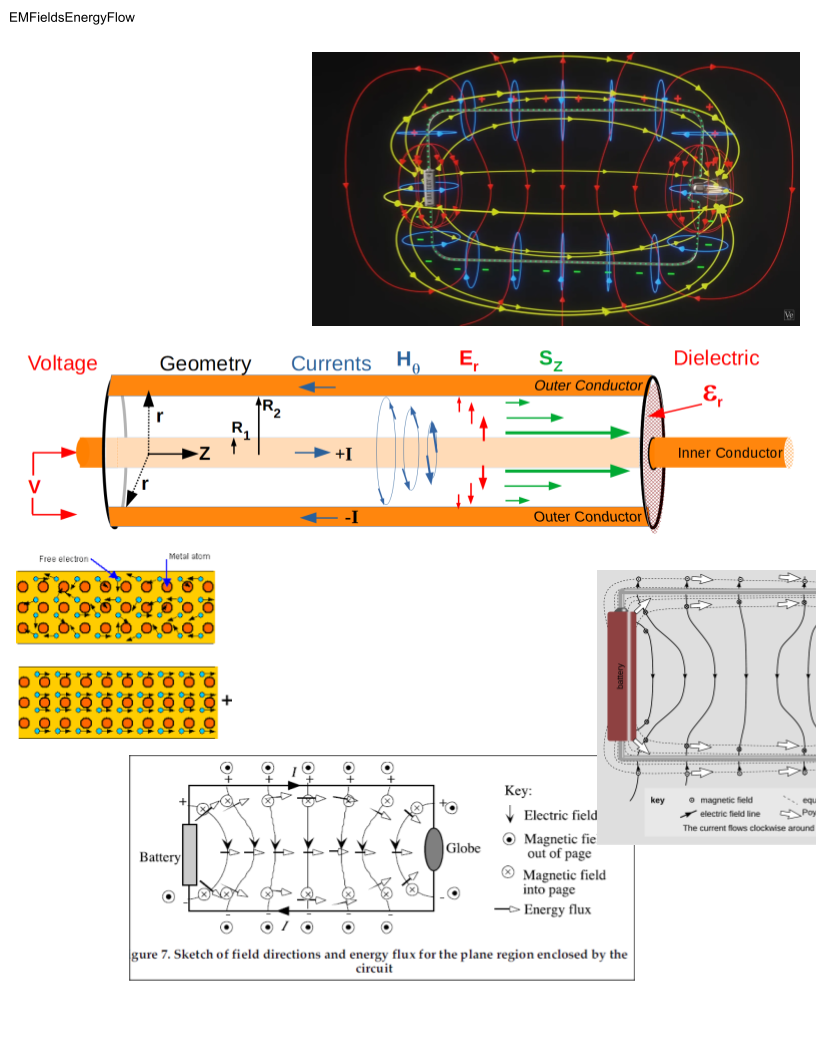
\includegraphics[width=\textwidth,height=\textheight,keepaspectratio]{04_EMFieldsEnergyFlow/em_illus.png}}
\end{figure}